Im Nachfolgenden soll die Funktechnologie auf der diese Arbeit aufbaut beschrieben werden. Long Range (LoRa) bildet dabei die Pysikalische schicht wärend das Long Range Wide Area Network (LoraWAN) die Netzwerkschicht übernimmt. Die genaue aufteilung kann der Abbildung \ref{fig:lora-lorawan-osi} entnommen werden.

\begin{figure}[H]
\centering
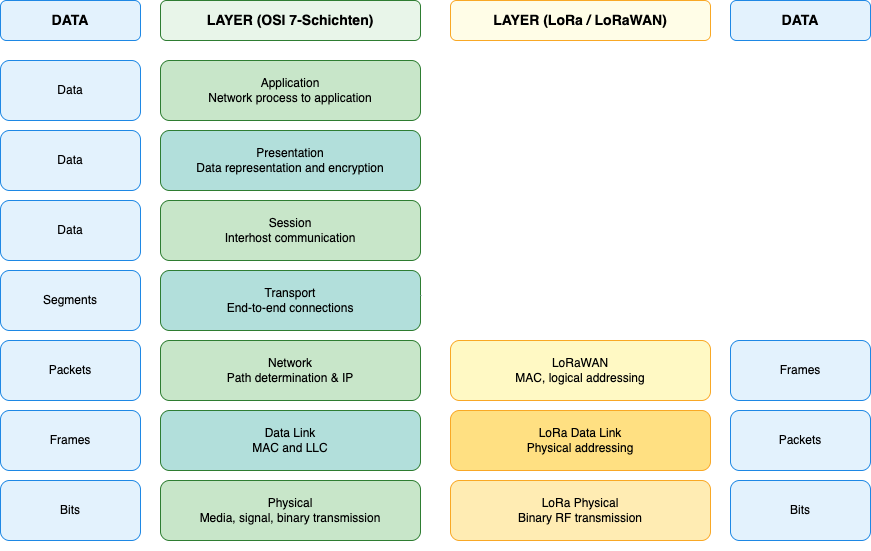
\includegraphics[scale=.4]{figures/diagrams/LoraWAN_OSI.png}
\caption{LoRa und LoRaWAN im OSI Schichtenmodell \ref{eckLoRaWANImDetail2019}}
\label{fig:lora-lorawan-osi}
\end{figure}

\subsubsection*{LoRa}

\paragraph*{Einordnung und Überblick}  
LoRa ist ein proprietäres und patentiertes drahtloses Übertragungsverfahren, das von der Semtech Corporation entwickelt wurde. 
Die Technologie arbeitet auf der physikalischen Schicht, auch Bitübertragungsschicht genannt, und basiert auf der Spread-Spectrum-Modulationstechnik \textit{Chirp Spread Spectrum} (CSS). 
Ziel von LoRa ist es, mit sehr geringem Energieverbrauch eine hohe Reichweite zu ermöglichen, auch unter schwierigen Ausbreitungsbedingungen. 

\paragraph*{Modulationstechnik}  
Chirp Spread Spectrum (CSS) ist ein Modulationsverfahren, bei dem die Frequenz des Signals während der Übertragungszeit kontinuierlich ansteigt oder abfällt.
Ein „Upchirp“ (Abbildung \ref{fig:lora-chirp} links) ist eine Erhöhung der Frequenz von niedrig nach hoch, während ein „Downchirp“ (Abbildung \ref{fig:lora-chirp} rechts) eine Absenkung der Frequenz von hoch nach niedrig darstellt. 

\begin{figure}[H]
\centering
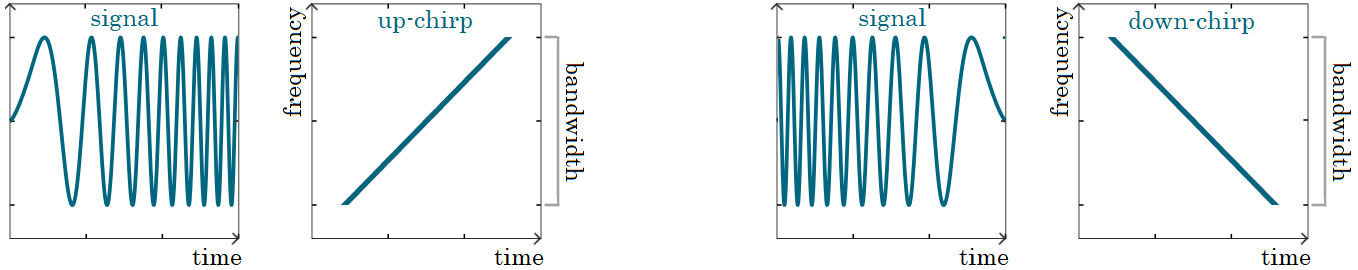
\includegraphics[scale=.4]{figures/asstes/lora-chirps.png}
\caption{LoRa Chirps \cite{tulkaLoRaSpreadingFactor}}
\label{fig:lora-chirp}
\end{figure}

Durch diese Methode wird das Datensignal über ein breiteres Frequenzband verteilt, wodurch es robust gegenüber Rauschen und Interferenzen wird.  
Ein wesentlicher Vorteil von CSS gegenüber anderen Modulationstechniken, wie z.\,B. der in Abschnitt \ref{sec:drahtlosedatenübertragung} genannten FSK, ist die Fähigkeit, Signale selbst dann zu dekodieren, wenn sie unterhalb des Rauschpegels liegen.



\paragraph*{Symbolstruktur und Datenübertragung}  
LoRa überträgt Daten in Symbolen, die die kleinste Informationseinheit darstellen. Ein Symbol fasst eine bestimmte Anzahl an Bits zusammen, deren Anzahl durch den sogenannten Spreading Factor (SF) bestimmt wird. Je höher der SF, desto mehr Bits pro Symbol und desto größer die Anzahl an möglichen Symbolwerten. \\

Der Spreading Factor (SF) ist ein zentraler Parameter der LoRa-Modulation. Er beschreibt das Verhältnis zwischen Chiprate und Symbolrate und bestimmt damit direkt die Datenrate $R_b$ eines Systems.  

\begin{equation}
\label{eq:spredigfactorbandwith}
R_b = \frac{SF \cdot B}{2^{SF}} \cdot \frac{4}{4 + CR},
\end{equation}

Wobei $B$ die Bandbreite und $CR$ der Codierungsfaktor ist \cite[S.6]{rhode&schwarzCharacterizationLoRaDevices}.  

Mit steigendem SF verlängert sich die Dauer eines Symbols, da der zugrunde liegende Chirp über eine größere Zeitspanne ausgesendet wird. Dadurch wird die Übertragung robuster gegenüber Rauschen und Störungen und erlaubt größere Reichweiten. Gleichzeitig sinkt jedoch die Datenrate, da weniger Symbole pro Zeiteinheit übertragen werden können. In der Praxis bedeutet das: Ein niedriger SF (z.\,B. SF7) ermöglicht eine hohe Datenrate, eignet sich aber nur für kurze Distanzen mit gutem Empfang, während ein hoher SF (z.\,B. SF12) sehr große Reichweiten erlaubt, jedoch nur eine geringe Datenrate bereitstellt. Der Spreading Factor stellt somit einen zentralen Kompromiss zwischen Reichweite und Datenrate dar. \\

Die Übertragung erfolgt nicht durch feste Töne oder Frequenzen wie beispielsweise bei FSK, sondern über das CSS Verfahren. Bei LoRa steigt die Frequenz während der Symboldauer linear an (Upchirp). Der jeweilige Startpunkt des Chirps auf der Frequenzachse wird dabei zyklisch verschoben und codiert so den Symbolwert. Jedes Symbol entspricht also einem verschobenen Chirp (siehe Abbildung \ref{fig:lora-symbole}). 

\begin{figure}[H]
\centering
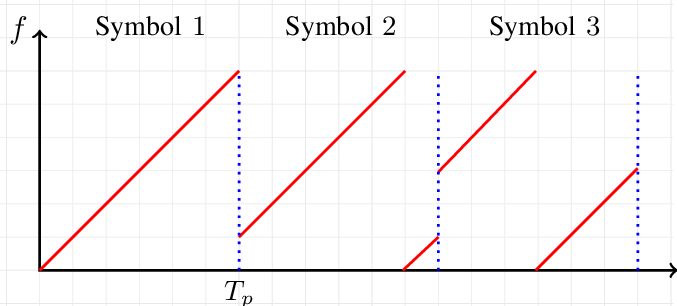
\includegraphics[scale=.4]{figures/asstes/n-LoRa-CSS-each-symbol-is-encoded-as-a-single-circularly-shifted-chirp-and-covers-the.png}
\caption{LoRa Symbole \cite{inproceedings}}
\label{fig:lora-symbole}
\end{figure} 

Beim Empfänger wird das Signal mit einem Referenz-Downchirp multipliziert. Dadurch wird aus dem verschobenen Chirp ein nahezu konstanter Ton, dessen Frequenz eindeutig dem gesendeten Symbolwert entspricht. Über eine diskrete Fourier-Transformation (DFT) lässt sich dieser Wert präzise bestimmen. So können auch Signale erkannt werden, die unterhalb des normalen Rauschpegels liegen. \autocite{tulkaLoRaSpreadingFactor, 8067462}

\paragraph*{Regulatorische Rahmenbedingungen (EU)}
In Europa wird das EU863–870-Band für LoRa verwendet mit \emph{Duty-Cycle}-Grenzen je Subband und Sendeleistungsgrenzen. Gerätekonfiguration und Kanalpläne folgen den \emph{LoRa Alliance Regional Parameters} (RP002), während die verbindlichen Funkparameter in \emph{ETSI EN~300~220} festgelegt sind. 
\autocite{RP002104, ETSIEN3002202025}

\paragraph*{Zusammenfassung}  
LoRa nutzt CSS als Modulationstechnik, wodurch eine robuste Datenübertragung selbst unter dem Rauschpegel möglich ist. 
Der Spreading Factor ist der zentrale Parameter, der Reichweite und Datenrate bestimmt. 
Die Datenübertragung erfolgt über symmetrische Chirp-Symbole, die durch Korrelation und Fourier-Analyse effizient erkannt werden können. 
Damit eignet sich LoRa besonders für Anwendungen mit geringer Datenrate, aber hoher Reichweitenanforderung. 


\subsubsection*{LoRaWAN} 
\label{sec:lorawan}

LPWANs (Low Power Wide Area Networks) ermöglichen energieeffiziente Kommunikation über große Distanzen und gelten daher als eine Schlüsseltechnologie für das Internet der Dinge (IoT). LoRaWAN zählt zu den vielversprechendsten LPWAN-Technologien. Es bietet geringe Leistungsaufnahme, niedrige Kosten und große Reichweite, geht jedoch mit einer geringen Datenrate einher. Während LoRa lediglich die physikalische Modulation beschreibt, definiert LoRaWAN (Long Range Wide Area Network) das darüberliegende Netzwerkprotokoll und die Architektur für die Kommunikation zwischen Endgeräten, Gateways und Netzwerkservern.

\paragraph*{LoRaWAN Netzwerkarchitektur}
Ein typisches LoRaWAN-Netzwerk besteht aus drei zentralen Komponenten. An erster Stelle stehen die Endgeräte, auch \textit{Nodes} genannt (in Abbildung \ref{fig:lorawan-architektur} unter \textit{End Nodes}). Dabei handelt es sich um Sensoren oder Aktoren, die Daten erfassen oder Befehle ausführen können. Diese Geräte besitzen keine direkte Internetanbindung, sondern lediglich einen LoRa-Chip sowie den LoRaWAN-Stack in ihrer Firmware. Alle Daten werden also über diese Schnittstelle empfangen oder gesendet.

Die zweite Komponente bilden die Gateways (in Abbildung \ref{fig:lorawan-architektur} unter \textit{Concentrator / Gateway}). Sie sind mit einem LoRa-Chip und einer aktiven Internetverbindung ausgestattet und fungieren als Schnittstelle zwischen der drahtlosen LoRa-Kommunikation und dem IP-Netzwerk. Sobald ein Gateway ein gültiges LoRaWAN-Paket empfängt, leitet es dieses an den Netzwerkserver weiter.

Der Netzwerkserver stellt die zentrale Instanz des gesamten LoRaWAN-Systems dar (in Abbildung \ref{fig:lorawan-architektur} unter \textit{Network Server}). Er filtert redundante Nachrichten, übernimmt die Authentifizierung und Sicherheit, steuert die Weiterleitung an die jeweiligen Anwendungsserver und verwaltet gleichzeitig die angebundenen Endgeräte \cite{LoRaWANArchitecture}.

\begin{figure}[H]
\centering
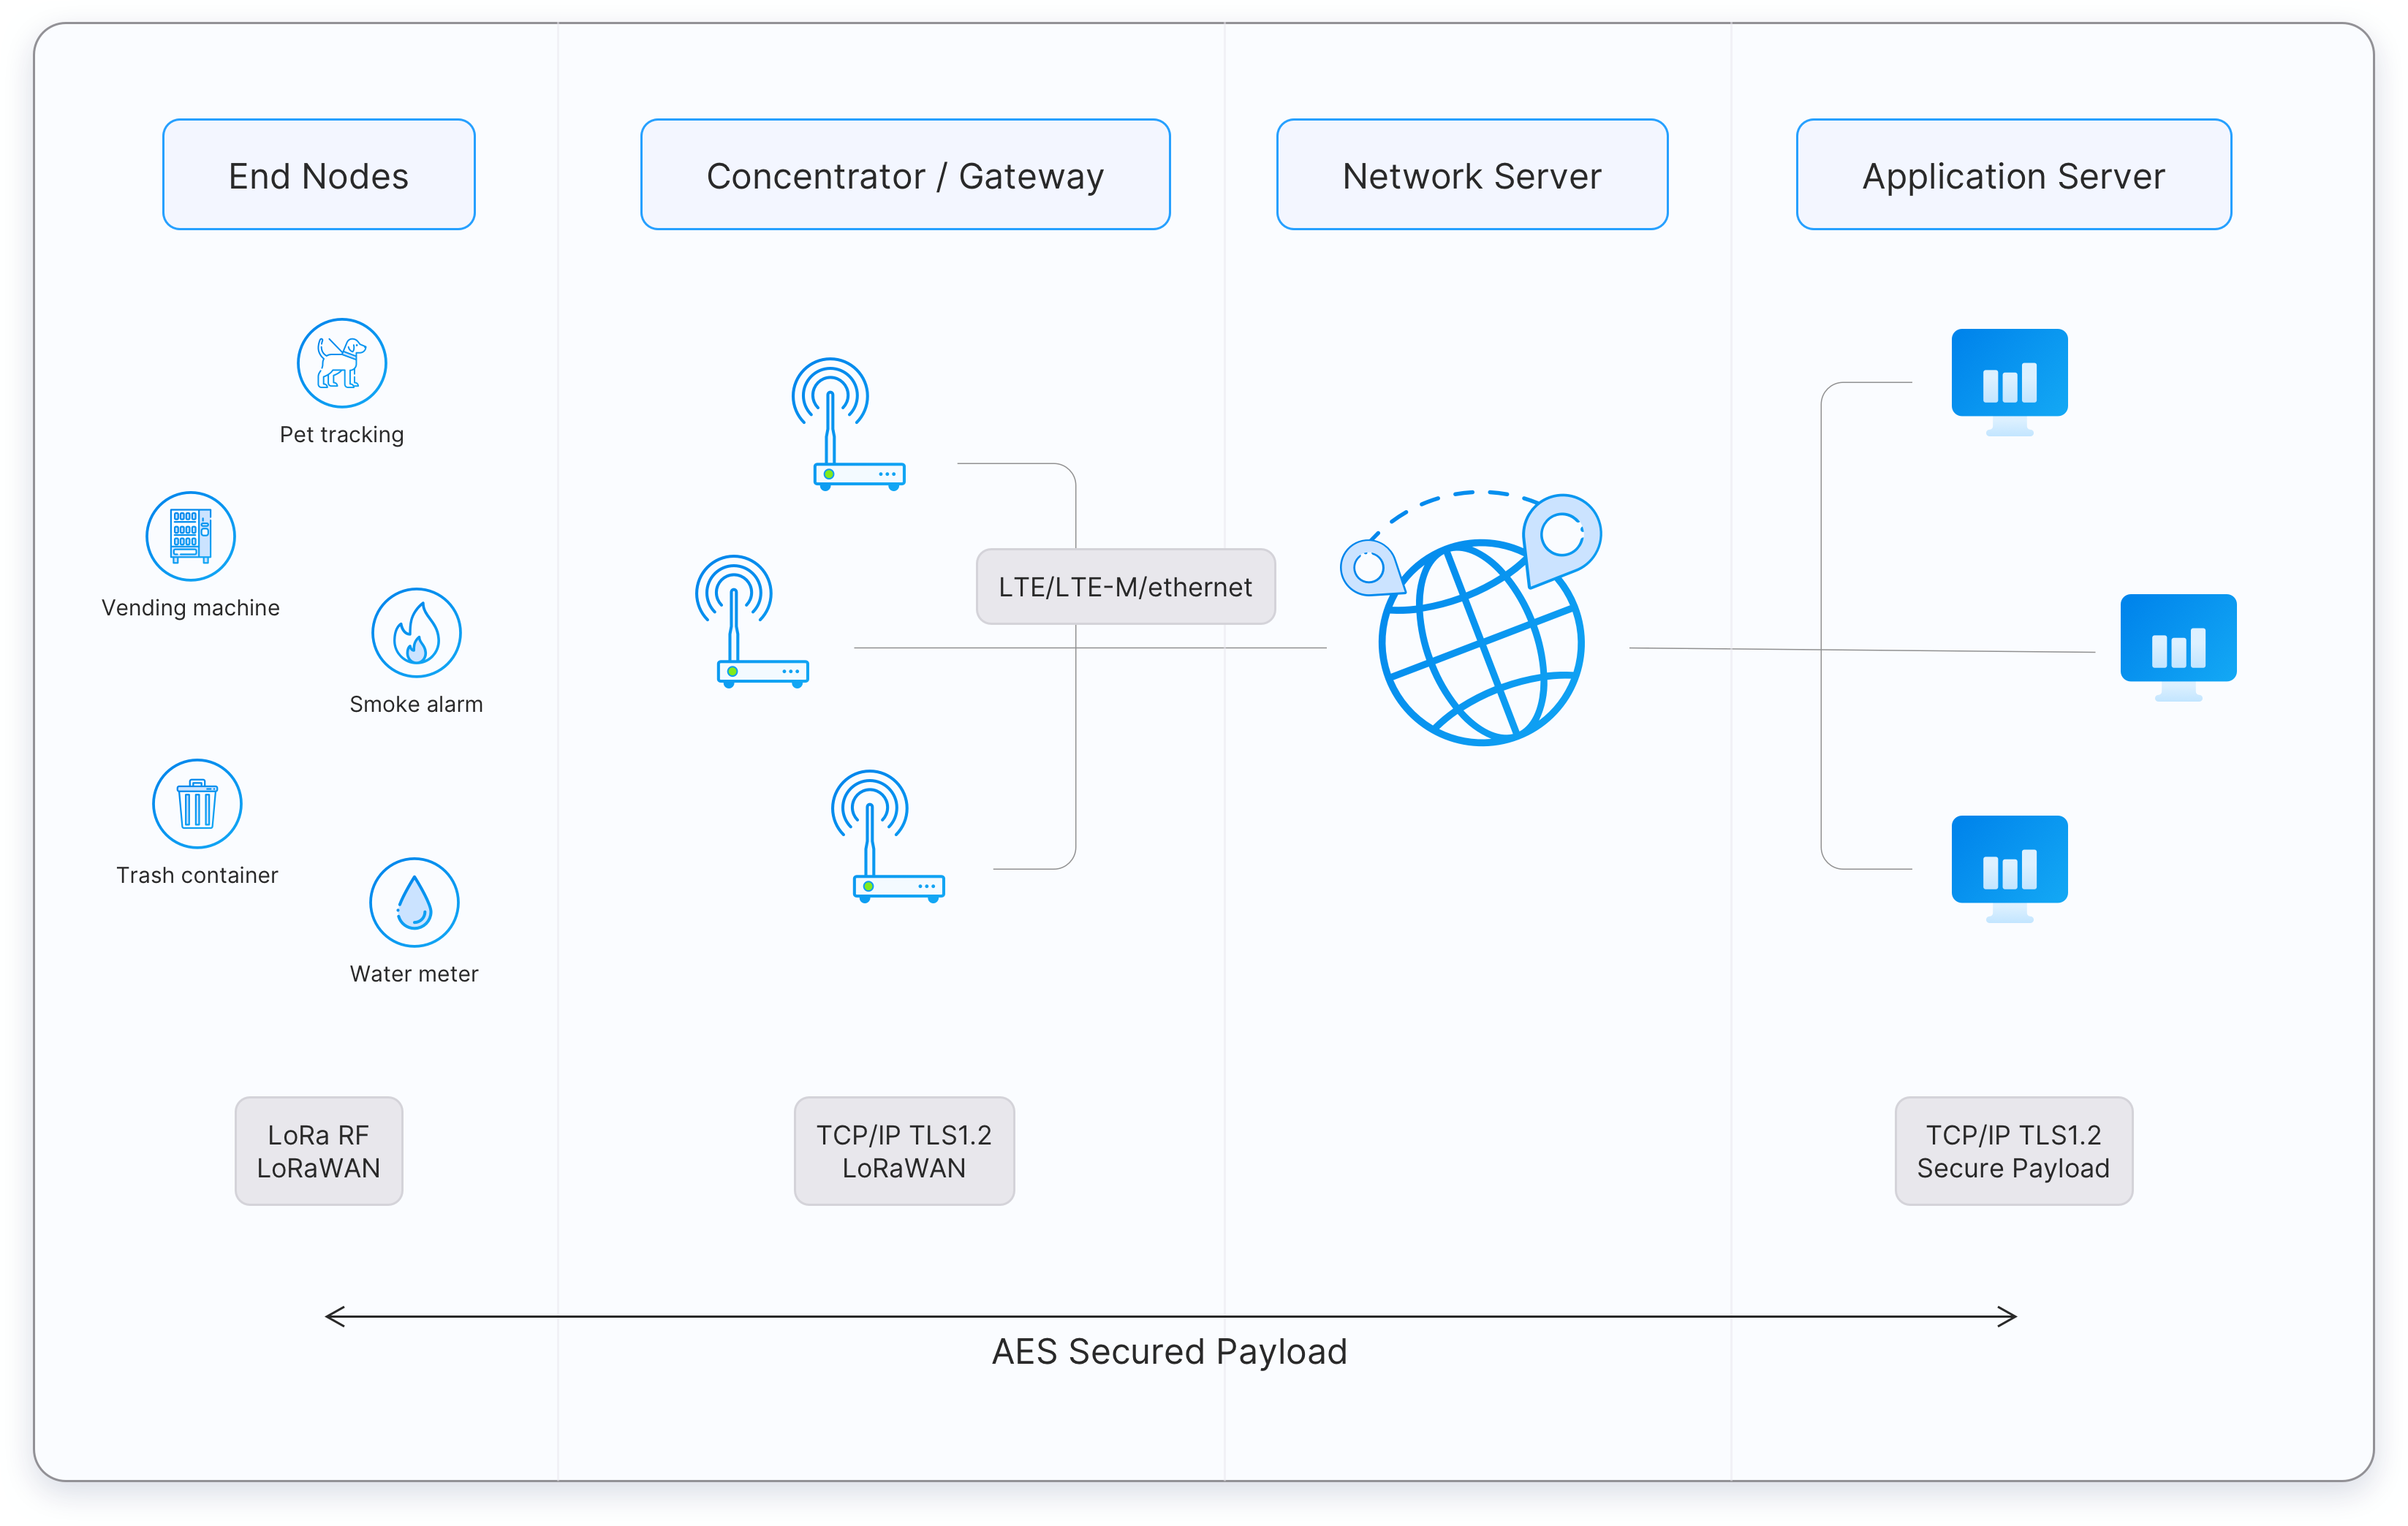
\includegraphics[scale=.135]{figures/asstes/lorawan-architecture.png}
\caption{LoRaWAN Architektur \cite{LoRaWANArchitecture}}
\label{fig:lorawan-architektur}
\end{figure} 

\paragraph*{LoRaWAN Geräteklassen}
LoRaWAN unterscheidet drei Gerätekategorien, die sich vor allem in ihren Energiesparmechanismen und Kommunikationsmöglichkeiten unterscheiden. Die energieeffizienteste Variante und zugleich die Mindestanforderung an ein LoRaWAN-Endgerät ist die Geräteklasse \textbf{A}. Sie eignet sich besonders für batteriebetriebene Systeme. Wie alle Klassen unterstützt auch Klasse A eine bidirektionale Kommunikation. Um den Energieverbrauch jedoch so gering wie möglich zu halten, können Downlink-Nachrichten vom Netzwerkserver nur kurz nach einem Uplink empfangen werden. Zu diesem Zweck öffnet das Endgerät nach jeder eigenen Übertragung zwei kurze Empfangsfenster (RX1 und RX2).

Die Geräteklasse \textbf{B} erweitert dieses Konzept um zusätzliche, periodische Empfangsfenster. Dadurch lassen sich Downlink-Nachrichten planbar zustellen. Jedes Gerät startet zunächst in Klasse A und kann vom Netzwerkserver in Klasse B versetzt werden, sofern es den entsprechenden Standard unterstützt.

Die dritte Kategorie ist die Geräteklasse \textbf{C}. Sie ist vor allem für netzbetriebene Geräte gedacht, da ihr Empfangsfenster (RX2) permanent geöffnet ist. Damit wird eine verzögerungsfreie Kommunikation zwischen Endgerät und Netzwerkserver möglich, was allerdings mit einem deutlich höheren Energieverbrauch verbunden ist \autocite{sornin2015lorawan}.

\paragraph*{LoRaWAN Join-Mechanismen}  
Damit ein Endgerät Nachrichten an ein LoRaWAN-Netzwerk senden kann, muss es sich zunächst anmelden. Hierfür existieren zwei grundlegende Verfahren: \textit{Over-The-Air Activation} (OTAA) und \textit{Activation by Personalization} (ABP).  

Bei OTAA, dem empfohlenen und sichersten Mechanismus, authentifiziert sich das Endgerät über einen Join-Vorgang beim Netzwerkserver. Das Gerät sendet dazu eine Join-Request-Nachricht, die unter anderem die eindeutige Gerätekennung \textit{DevEUI} sowie eine eindeutige Anwendungskennung enthält. In LoRaWAN v1.0.x wird diese als \textit{AppEUI} bezeichnet, während ab v1.1 der Begriff \textit{JoinEUI} verwendet wird. Zusätzlich wird ein \textit{DevNonce} übertragen, ein einmaliger Wert, der sicherstellt, dass Join-Nachrichten nicht wiederverwendet werden können, um Replay-Angriffe zu verhindern. Die Join-Nachricht ist zwar unverschlüsselt, jedoch mit einem MIC (Message Integrity Code) abgesichert.  

Nach erfolgreicher Prüfung sendet der Netzwerkserver eine Join-Accept-Nachricht zurück, die weitere Parameter wie \textit{NetID}, \textit{DevAddr} sowie Nonces für die Schlüsselerzeugung enthält. Anschließend werden die Sitzungsschlüssel abgeleitet. In LoRaWAN v1.0.x entstehen aus dem geheimen \textit{AppKey} zwei Session Keys, nämlich der \textit{NwkSKey} für die Netzwerkschicht und der \textit{AppSKey} für die Anwendungsschicht. Ab Version 1.1 unterscheidet LoRaWAN stärker zwischen Netzwerk- und Anwendungsebene. Hier wird der \textit{AppSKey} weiterhin aus dem \textit{AppKey} erzeugt, während drei verschiedene Netzwerkschlüssel (\textit{FNwkSIntKey}, \textit{SNwkSIntKey} und \textit{NwkSEncKey}) aus einem separaten \textit{NwkKey} abgeleitet werden. Durch diese Trennung wird die Sicherheit und Flexibilität bei der Schlüsselverwaltung erhöht.  

Im Gegensatz dazu verzichtet ABP vollständig auf einen Join-Prozess. Die für die Kommunikation erforderlichen Parameter, also die Geräteadresse \textit{DevAddr} sowie die Session Keys, werden hierbei direkt im Gerät vorkonfiguriert und auch im Netzwerkserver hinterlegt. In LoRaWAN v1.0.x handelt es sich dabei um den \textit{NwkSKey} und den \textit{AppSKey}, während ab Version 1.1 zusätzlich die drei Netzwerkschlüssel \textit{FNwkSIntKey}, \textit{SNwkSIntKey} und \textit{NwkSEncKey} berücksichtigt werden müssen. ABP ermöglicht somit eine sofortige Nutzung des Netzwerks, bietet jedoch geringere Sicherheit, da die Schlüssel statisch sind und nicht regelmäßig erneuert werden.  

Zusammenfassend bietet OTAA durch die dynamische Erzeugung von Sitzungsschlüsseln bei jedem Join deutlich mehr Sicherheit und Flexibilität, während ABP vor allem für Testaufbauten oder spezielle Szenarien mit festen Parametern genutzt wird.  

\paragraph*{Leistungsmerkmale und Herausforderungen}
LoRaWAN kann durch Parameteroptimierung an unterschiedliche Anwendungen angepasst werden. Wichtige Designaspekte sind Skalierbarkeit, Durchsatz, Abdeckung, Energieeffizienz und geringe Kosten \cite{bor2017lora}. Herausforderungen bestehen insbesondere in:

\begin{itemize}
    \item \textbf{Skalierbarkeit:} Beeinflusst durch Faktoren wie verfügbare Kanäle, Spreizfaktor, Bandbreite und regulatorische Einschränkungen. In Europa steht für LoRa das Band von 863 MHz bis 870 MHz zur Verfügung, in Amerika von 902 MHz bis 928 MHz \autocite{FrequencyPlans}.
    
    \item \textbf{Energieeinsparung:} Durch die Adaptive Data Rate (ADR) oder eine optimierte Parameterwahl kann der Energieverbrauch zusätzlich reduziert werden \autocite{kufakunesuSurveyAdaptiveData2020}.
    
    \item \textbf{Sicherheit:} LoRaWAN setzt auf Ende-zu-Ende-Verschlüsselung mit einer klaren Aufgabentrennung zwischen Join Server, Network Server und Application Server. Damit werden Schlüssel sicher verwaltet, Betreiber erhalten nur die für sie notwendigen Informationen, und Multi-Tenant-Szenarien werden unterstützt. Neuere Spezifikationen (ab v1.1) verbessern zudem die Schlüsselverwaltung durch die Trennung von Anwendungs- und Netzwerkschlüsseln \autocite{butun2019security,LoRaWANBackendInterfaces11}.
\end{itemize}

\paragraph*{Anwendungsgebiete}
LoRaWAN eignet sich für zahlreiche IoT-Szenarien, darunter smarte digitale Städte, smarte Messungen (z.\,B. für Pflanzen), intelligentes Parkraummanagement oder adaptive Straßenbeleuchtung \autocite{BadenWuerttembergFoerdertLong2024}. Aufgrund der niedrigen Bitrate ist der Einsatz jedoch auf Anwendungen mit geringer Datenübertragungsrate beschränkt.

\paragraph*{Roaming, Peering und Interoperabilität}
LoRaWAN-Roaming erlaubt es, dass Endgeräte auch außerhalb des eigenen Netzwerks funktionieren können. Es gibt zwei Arten von Roaming:

\begin{itemize}
  \item \textbf{Passives Roaming:} Das Endgerät bleibt unter der Kontrolle seines Heimat-Netzservers (Serving NS), die Funkverbindung läuft aber über fremde Gateways und Netzserver (Forwarding NS). Diese leiten die Daten nur weiter, ohne die eigentliche Gerätesteuerung zu übernehmen.
  \item \textbf{Handover Roaming:} Hier übergibt der Heimat-Netzserver die Kontrolle an einen besuchten Netzserver (Serving NS). Dieser steuert dann das Endgerät aktiv, während der Heimat-NS im Hintergrund für die Schlüsselaushandlung und Verwaltung eingebunden bleibt.
\end{itemize}

Damit Roaming überhaupt funktioniert, müssen Netzbetreiber Peering- oder Roamingabkommen schließen. 
\emph{Packet Broker} bietet dazu ein globales Vermittlungsnetz, das den Austausch von Paketen zwischen verschiedenen Betreibern erleichtert. Ein Beispiel ist das offene Netz \texttt{The Things Network (TTN)} mit der \texttt{NetID~000013}. 

Kommerzielle Anbieter wie Senet setzen zusätzlich auf bilaterale Roaming-Vereinbarungen mit Partnernetzen, um ihre Abdeckung zu erweitern. \cite{LoRaWANBackendInterfaces11,PacketBroker,TTNNetID,SenetExt}